\section{Условие задания}

\begin{figure}[H]
    \begin{center}
        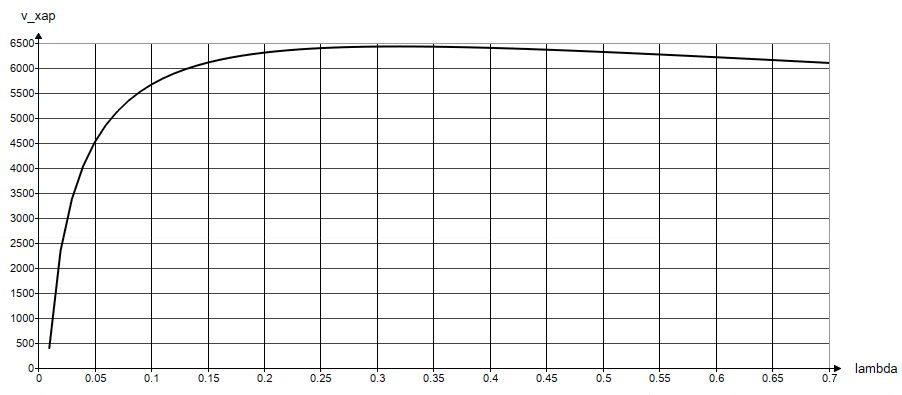
\includegraphics[width = 0.5\linewidth]{pic1.PNG}
        \caption{Условие задания}
        \label{pic1}
    \end{center} 
\end{figure}

\section{Решение}

В данном задании нагрузка симметрична относительно оси $y$. Выберем отсчет угла $\phi$ от этой оси. Также разобьем кольцо на 2 участка. Один участок содержит распределенную нагрузку $q_0$ и уравновешивающую силу $t$, другой --- только уравновешивающую силу $t$.

\begin{figure}[H]
    \begin{center}
        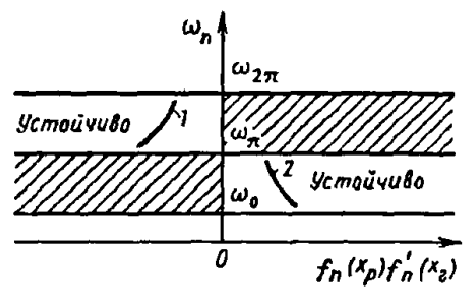
\includegraphics[width = 0.5\linewidth]{pic2.PNG}
        \caption{Расчетная схема}
        \label{pic2}
    \end{center}
\end{figure}

Уравновешивающую силу $t$ будем искать в виде 
\begin{equation}
    \label{eq1}
    t = A + B \cos \phi + C \sin \phi
\end{equation}

Рассмотрим равновесие кольца вдоль оси $y$:
\begin{equation}
    \label{eq2}
    \Sigma F_y = 0
\end{equation}
\begin{equation}
    \label{eq3}
    \oint (A + B \cos \phi + C \sin \phi) \sin \phi R d \phi - 2q_0R - 2 \int_{0}^{\frac{\pi}{2}} {q_0R \cos \phi d \phi} = 0
\end{equation}

Интегралы от выражений $A \sin \phi$ и $B \cos \phi \sin \phi$ по замкнутому контуру дадут 0.
\begin{equation}
    \label{eq4}
    \int_{0}^{2 \pi}{C \sin^2 \phi R d \phi} - 2q_0R - 2q_0R \int_{0}^{\frac{\pi}{2}}{\cos \phi d \phi} = 0
\end{equation}
\begin{equation}
    \label{eq5}
    CR \cdot \frac{1}{2}(\phi - \sin 2 \phi) |_{\phi=0}^{2 \pi} - 2q_0R - 2q_0R \sin \phi |_{\phi = 0}^{\frac{\pi}{2}} = 0
\end{equation}
\begin{equation}
    \label{eq6}
    \pi CR - 2q_0R - 2q_0R = 0
\end{equation}
\begin{equation}
    \label{eq7}
    C = \frac{4q_0}{\pi}
\end{equation}

Получим выражение для $t$:
\begin{equation}
    \label{eq8}
    t = \frac{4q_0}{\pi} \sin \phi
\end{equation}

Запишем общие выражения для уравнений равновесия:
\begin{equation}
    \label{eq9}
    \begin{cases}
        \displaystyle \frac{d^2 Q}{d \phi^2} + Q = R(t + \frac{dQ}{d \phi})
        \\[10pt]
        \displaystyle \frac{dM}{d \phi} = R(Q + m)
        \\[10pt]
        \displaystyle N = -\frac{dQ}{d \phi} + qR
    \end{cases}
\end{equation}

Запишем уравнения (\ref{eq9}) для первого участка:
\begin{equation}
    \label{eq10}
    \begin{cases}
        \displaystyle \frac{d^2 Q_1}{d \phi^2} + Q_1 = \frac{4q_0}{\pi} R \sin \phi
        \\[10pt]
        \displaystyle \frac{dM_1}{d \phi} = RQ_1
        \\[10pt]
        \displaystyle N_1 = - \frac{dQ_1}{d \phi} + q_0R
    \end{cases}
\end{equation} 

Для второго участка:
\begin{equation}
    \label{eq11}
    \begin{cases}
        \displaystyle \frac{d^2Q_2}{d \phi^2} + Q_2 = \frac{4q_0}{\pi} R \sin \phi
        \\[10pt]
        \displaystyle \frac{dM_2}{d \phi} = RQ_2
        \\[10pt]
        \displaystyle N_2 = - \frac{dQ_2}{d \phi}
    \end{cases}
\end{equation}

Решим систему уравнений (\ref{eq10}):
\begin{equation}
    \label{eq12}
    Q_1 = Q_{10} + Q_1^* = C_1 \cos \phi + C_2 \sin \phi - \frac{2q_0}{\pi} R\phi \cos \phi
\end{equation}
\begin{equation}
    \label{eq13}
    \begin{split}
        M_1 & = \int{RQ_1 d \phi} = R \int{(C_1 \cos \phi + C_2 \sin \phi - \frac{2q_0}{\pi}R \phi \cos \phi) d \phi} =
        \\
        & = R (C_1 \sin \phi - C_2 \cos \phi - \frac{2q_0}{\pi}R (\phi \sin \phi + \cos \phi)) + C_3
    \end{split}
\end{equation}
\begin{equation}
    \label{eq14}
    N_1 = C_1 \sin \phi - C_2 \cos \phi + \frac{2q_0}{\pi} R (\cos \phi - \phi \sin \phi) + q_0R
\end{equation}

и систему уравнений (\ref{eq11}):
\begin{equation}
    \label{eq15}
    Q_2 = Q_{20} + Q_2^* = C_4 \cos \phi + C_5 \sin \phi - \frac{2q_0}{\pi} R\phi \cos \phi
\end{equation}
\begin{equation}
    \label{eq16}
    \begin{split}
        M_2 & = \int{RQ_2 d \phi} = R \int{(C_4 \cos \phi + C_5 \sin \phi - \frac{2q_0}{\pi}R \phi \cos \phi) d \phi} =
        \\
        & = R (C_4 \sin \phi - C_5 \cos \phi - \frac{2q_0}{\pi}R (\phi \sin \phi + \cos \phi)) + C_6
    \end{split}
\end{equation}
\begin{equation}
    \label{eq17}
    N_2 = C_4 \sin \phi - C_5 \cos \phi + \frac{2q_0}{\pi} R (\cos \phi - \phi \sin \phi)
\end{equation}

Воспользуемся свойством симметрии: при симметричной нагрузке кососимметричные факторы на оси симметрии равны нулю.
\begin{equation}
    \label{eq18}
    \phi = 0: \; Q_1 = 0 => C_1 = 0
\end{equation}
\begin{equation}
    \label{eq19}
    \phi = \pi: \; Q_2 = 0
\end{equation}
\begin{equation}
    \label{eq20}
    -C_4 + 2q_0R = 0 => C_4 = 2q_0R
\end{equation}

Получим следующие выражения для силовых факторов:
\begin{equation}
    \label{eq21}
    \begin{cases}
        \displaystyle Q_1 = C_2 \sin \phi - \frac{2q_0}{\pi}R \phi \cos \phi
        \\[10pt]
        \displaystyle M_1 = - C_2 R \cos \phi - \frac{2q_0}{\pi}R^2 (\phi \sin \phi + \cos \phi) + C_3
        \\[10pt]
        \displaystyle N_1 = - C_2 \cos \phi + \frac{2q_0}{\pi}R (\cos \phi - \phi \sin \phi) + q_0 R
    \end{cases}
\end{equation}
\begin{equation}
    \label{eq22}
    \begin{cases}
        \displaystyle Q_2 = C_5 \sin \phi + 2q_0 R (\cos \phi - \frac{1}{\pi}\phi \cos \phi)
        \\[10pt]
        \displaystyle M_2 = -C_5 R \cos \phi + 2q_0R^2 (\sin \phi - \frac{1}{\pi} (\phi \sin \phi + \cos \phi)) + C_6
        \\[10pt]
        \displaystyle N_2 = - C_5 \cos \phi + 2q_0 R (\sin \phi + \frac{1}{\pi} (\cos \phi - \phi \sin \phi))
    \end{cases}
\end{equation}

Рассмотрим стык 2-х участков:
\begin{figure}[H]
    \begin{center}
        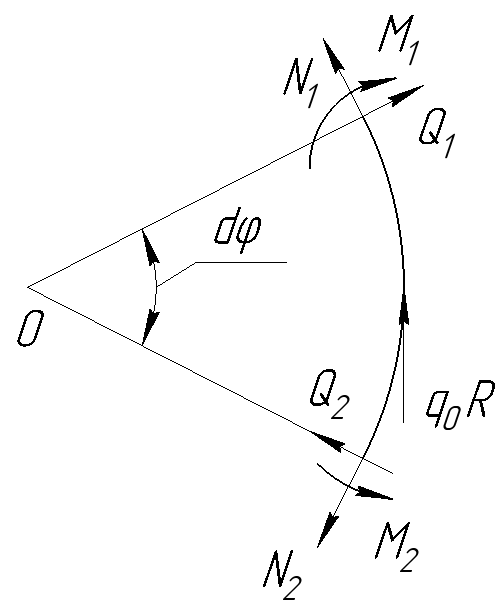
\includegraphics[width = 0.5\linewidth]{pic3.PNG}
        \caption{Стык 2-х участков}
        \label{pic3}
    \end{center}
\end{figure}

Запишем условия его равновесия:
\begin{equation}
    \label{eq23}
    Q_1 = Q_2
\end{equation}
\begin{equation}
    \label{eq24}
    M_1 = M_2
\end{equation}
\begin{equation}
    \label{eq25}
    N_1 + q_0R = N_2
\end{equation}

Из уравнения (\ref{eq23}) получим:
\begin{equation}
    \label{eq26}
    C_2 = C_5
\end{equation}

Из уравнения (\ref{eq24}) получим:
\begin{equation}
    \label{eq27}
    - \frac{2q_0}{\pi}R^2 \cdot \frac{\pi}{2} + C_3 = 2q_0R^2 (1 - \frac{1}{\pi} \cdot \frac{\pi}{2})
\end{equation}
\begin{equation}
    \label{eq28}
    - q_0R^2 + C_3 = q_0R^2 + C_6
\end{equation}
\begin{equation}
    \label{eq29}
    C_3 = C_6 + 2q_0R^2
\end{equation}

Из уравнения (\ref{eq25}) получим:
\begin{equation}
    \label{eq30}
    - \frac{2q_0}{\pi}R \cdot \frac{\pi}{2} + q_0R + q_0R = 2q_0R (1 - \frac{1}{\pi} \cdot \frac{\pi}{2})
\end{equation}
\begin{equation}
    \label{eq31}
    q_0R \equiv q_0R
\end{equation}

Для нахождения констант интегрирования воспользуемся интегральными соотношениями:
\begin{enumerate}
    \item $\oint M d \phi = 0$
    \begin{equation}
        \label{eq32}
        2 \int_{0}^{\pi}{M d \phi} = 0
    \end{equation}
    \begin{equation}
        \label{eq33}
        \int_{0}^{\frac{\pi}{2}}{M_1 d \phi} + \int_{\frac{\pi}{2}}^{\pi}{M_2 d \phi} = 0
    \end{equation}
    \begin{equation}
        \label{eq34}
        \begin{split}
            & \int_{0}^{\frac{\pi}{2}}{(-C_2R \cos \phi - \frac{2q_0}{\pi}R^2 (\phi \sin \phi + \cos \phi) + C_3)d \phi} +
            \\
            + & \int_{\frac{\pi}{2}}^{\pi}{(-C_5R \cos \phi + 2q_0R^2 (\sin \phi - \frac{1}{\pi}(\phi \sin \phi + \cos \phi)) + C_6)d \phi} = 0
        \end{split}
    \end{equation}
    \begin{equation}
        \label{eq35}
        \begin{split}
            & (-C_2R \sin \phi - \frac{2q_0}{\pi}R^2(2\sin \phi - \phi \cos \phi) + C_3 \phi) |_{\phi = 0}^\frac{\pi}{2} +
            \\
            + & (-C_5R \sin \phi + 2q_0R^2 (-\cos \phi - \frac{1}{\pi} (2\sin \phi - \phi \cos \phi)) + C_6 \phi) |_{\phi = \frac{\pi}{2}}^\pi = 0
        \end{split}
    \end{equation}
    \begin{equation}
        \label{eq36}
        -C_2R - \frac{4q_0}{\pi}R^2 + C_3 \frac{\pi}{2} + C_5R + 2q_0R^2 + \frac{2q_0}{\pi}R^2 (-\pi + 2) + C_6 \frac{\pi}{2} = 0
    \end{equation}
    \begin{equation}
        \label{eq37}
        -C_2R + C_3 \frac{\pi}{2} + C_5R + C_6 \frac{\pi}{2} = 0
    \end{equation}
    \begin{equation}
        \label{eq38}
        C_3 \frac{\pi}{2} + C_6 \frac{\pi}{2} = 0
    \end{equation}
    Откуда
    \begin{equation}
        \label{eq39}
        C_3 + C_6 = 0
    \end{equation}
    Из выражений (\ref{eq39}) и (\ref{eq29}) получим:
    \begin{equation}
        \label{eq40}
        \begin{cases}
            C_3 = q_0R^2
            \\
            C_6 = -q_0R^2
        \end{cases}
    \end{equation}
    Тогда уравнения (\ref{eq21}) и (\ref{eq22}) примут вид:
    \begin{equation}
        \label{eq41}
        \begin{cases}
            \displaystyle Q_1 = C_2 \sin \phi - \frac{2q_0}{\pi}R \phi \cos \phi
            \\[10pt]
            \displaystyle M_1 = - C_2 R \cos \phi - \frac{2q_0}{\pi}R^2 (\phi \sin \phi + \cos \phi) + q_0R^2
            \\[10pt]
            \displaystyle N_1 = - C_2 \cos \phi + \frac{2q_0}{\pi}R (\cos \phi - \phi \sin \phi) + q_0 R
        \end{cases}
    \end{equation}
    \begin{equation}
        \label{eq42}
        \begin{cases}
            \displaystyle Q_2 = C_5 \sin \phi + 2q_0 R (\cos \phi - \frac{1}{\pi}\phi \cos \phi)
            \\[10pt]
            \displaystyle M_2 = -C_5 R \cos \phi + 2q_0R^2 (\sin \phi - \frac{1}{\pi} (\phi \sin \phi + \cos \phi)) - q_0R^2
            \\[10pt]
            \displaystyle N_2 = - C_5 \cos \phi + 2q_0 R (\sin \phi + \frac{1}{\pi} (\cos \phi - \phi \sin \phi))
        \end{cases}
    \end{equation}
    \item $\oint M \cos \phi d \phi = 0$
    \begin{equation}
        \label{eq43}
        \int_{0}^{\frac{\pi}{2}}{M_1 \cos \phi d \phi} + \int_{\frac{\pi}{2}}^{\pi}{M_2 \cos \phi d \phi} = 0
    \end{equation}
    \begin{equation}
        \label{eq44}
        \begin{split}
            & \int_{0}^{\frac{\pi}{2}}{(-C_2R \cos^2 \phi - \frac{2q_0}{\pi}R^2 (\phi \sin \phi \cos \phi + \cos^2 \phi) + q_0R^2 \cos \phi)d \phi} +
            \\
            + & \int_{\frac{\pi}{2}}^{\pi}{(-C_5R \cos^2 \phi + 2q_0R^2 (\sin \phi \cos \phi - \frac{1}{\pi}(\phi \sin \phi \cos \phi + \cos^2 \phi)) - q_0R^2 \cos \phi)d \phi} = 0
        \end{split}
    \end{equation}
    \begin{equation}
        \label{eq45}
        \begin{split}
            & (-C_2R(\frac{\phi}{2} + \frac{1}{4} \sin 2\phi) - \frac{2q_0}{\pi}R^2(-\frac{\phi}{4} \cos 2\phi + \frac{1}{8} \sin 2\phi + \frac{\phi}{2} + \frac{1}{4}\sin 2\phi) + q_0R^2 \sin \phi) \big|_{\phi = 0}^{\frac{\pi}{2}} +
            \\
            + & (-C_5R(\frac{\phi}{2} + \frac{1}{4} \sin 2\phi) + 
            \\
            + & 2q_0R^2(-\frac{1}{4}\cos 2\phi - \frac{1}{\pi}(-\frac{\phi}{4} \cos 2\phi + \frac{1}{8} \sin 2\phi + \frac{\phi}{2} + \frac{1}{4} \sin 2\phi)) - q_0R^2 \sin \phi) \big|_{\phi = \frac{\pi}{2}}^\pi = 0
        \end{split}
    \end{equation}
    \begin{equation}
        \label{eq46}
        -C_2R \cdot \frac{\pi}{4} - \frac{2q_0}{\pi}R^2 \cdot (\frac{\pi}{8} + \frac{\pi}{4}) + q_0R^2 - C_5R \frac{\pi}{4} - q_0R^2 - \frac{2q_0}{\pi}R^2 (-\frac{3\pi}{8} + \frac{\pi}{4}) + q_0R^2 = 0
    \end{equation}
    \begin{equation}
        \label{eq47}
        -C_2R \frac{\pi}{4} - \frac{3}{4}q_0R^2 + q_0R^2 - C_5R \frac{\pi}{4} + \frac{1}{4}q_0R^2 = 0
    \end{equation}
    \begin{equation}
        \label{eq48}
        (C_2 + C_5)R \frac{\pi}{4} = \frac{q_0R^2}{2}
    \end{equation}
    \begin{equation}
        \label{eq48.1}
        C_2 + C_5 = \frac{2q_0R}{\pi}
    \end{equation}
    \begin{equation}
        \label{eq49}
        C_2 = C_5 = \frac{q_0R}{\pi}
    \end{equation}
\end{enumerate}

Получим итоговые выражения для силовых факторов:
\begin{equation}
    \label{eq50}
    \begin{cases}
        \displaystyle Q_1 = \frac{q_0R}{\pi}(\sin \phi - 2\phi \cos \phi)
        \\[10pt]
        \displaystyle M_1 = q_0R^2(1 - \frac{3}{\pi} \cos \phi - \frac{2}{\pi} \phi \sin \phi)
        \\[10pt]
        \displaystyle N_1 = q_0R(1 - \frac{2}{\pi} \phi \sin \phi + \frac{1}{\pi} \cos \phi)
    \end{cases}
\end{equation}
\begin{equation}
    \label{eq51}
    \begin{cases}
        \displaystyle Q_2 = q_0R (\frac{1}{\pi} \sin \phi + 2\cos \phi - \frac{2}{\pi} \phi \cos \phi)
        \\[10pt]
        \displaystyle M_2 = q_0R^2 (2 \sin \phi - \frac{3}{\pi} \cos \phi - \frac{2}{\pi}\phi \sin \phi - 1)
        \\[10pt]
        \displaystyle N_2 = q_0R (2\sin \phi - \frac{2}{\pi} \phi \sin \phi + \frac{1}{\pi}\cos \phi)
    \end{cases}
\end{equation}

Построим эпюры:
\begin{figure}[H]
    \begin{center}
        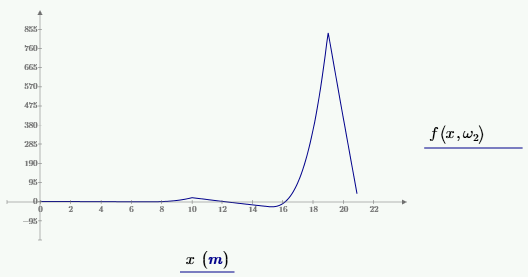
\includegraphics[width = 0.5\linewidth]{pic4.PNG}
        \caption{Эпюра перерезывающей силы $Q$}
        \label{pic4}
    \end{center}
\end{figure}
\begin{figure}[H]
    \begin{center}
        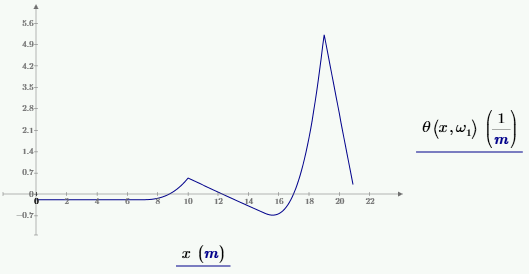
\includegraphics[width = 0.5\linewidth]{pic5.PNG}
        \caption{Эпюра изгибающего момента}
        \label{pic5}
    \end{center}
\end{figure}
\begin{figure}[H]
    \begin{center}
        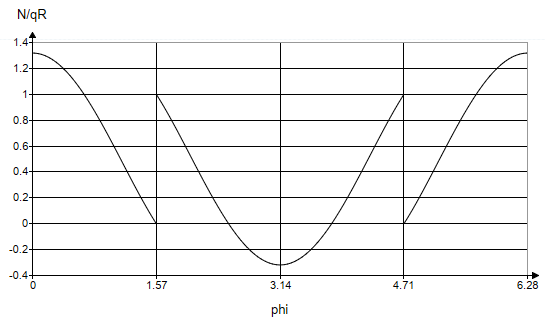
\includegraphics[width = 0.5\linewidth]{pic6.PNG}
        \caption{Эпюра нормальной силы}
        \label{pic6}
    \end{center}
\end{figure}